\documentclass{standalone}
\usepackage[utf8]{inputenc}
\usepackage{tikz}
\usetikzlibrary{shapes, arrows, arrows.meta, positioning, fit, calc}
\usepackage{pgfplots,pgfplotstable}
\pgfplotsset{compat=1.8}

% % This tex, loads the Breast GT pallete if is not defined.
% The document takes advantage of the xcolor package primitive 
% \def\@ifundefinedcolor#1{\@ifundefined{\string\color@#1}}
% therefore it xcolor package is needed or the definitions needs to be added.
% 
% TODO: 
% 	create a more generic script that checks if all the packages are there otherwise loads them.
%	or defines the missing primitive.
%   take a look at: \@ifpackageloaded{<name>}{<true>}{<false>}
% 					http://tex.stackexchange.com/questions/16199/test-if-a-package-or-package-option-is-loaded

\makeatletter
\newcommand{\colorprovide}[2]{%
  \@ifundefinedcolor{#1}{\colorlet{#1}{#2}}{}}

\newcommand{\defineColorWhenNoExist}[3]{%
  \@ifundefinedcolor{#1}{\definecolor{#1}{#2}{#3}}{}}
\makeatother

\defineColorWhenNoExist{bgColor}{rgb}{0.0000, 0.0000, 0.0000}
\defineColorWhenNoExist{boundaryColor}{rgb}{0.8784, 0.8784, 0.7529}
\defineColorWhenNoExist{chestWallColor}{rgb}{0.5294, 0.7843, 0.6078}
\defineColorWhenNoExist{fatColor}{rgb}{0.9804, 0.5882, 0.1176}
\defineColorWhenNoExist{fibroGlandColor}{rgb}{1.0000, 1.0000, 0.0000}
\defineColorWhenNoExist{lesionColor}{rgb}{1.0000, 0.2510, 0.0000}
\defineColorWhenNoExist{lungColor}{rgb}{0.2353, 0.6078, 0.8235}
\defineColorWhenNoExist{pectoralColor}{rgb}{0.6510, 0.3490, 1.0000}
\defineColorWhenNoExist{ribColor}{rgb}{0.0000, 0.4510, 0.1961}
\defineColorWhenNoExist{skinColor}{rgb}{0.9804, 0.7255, 0.7451}
\defineColorWhenNoExist{unkTissueColor}{rgb}{0.6000, 0.3020, 0.2510}


\newenvironment{customlegend}[1][]{%
    \begingroup
    % inits/clears the lists (which might be populated from previous
    % axes):
    \csname pgfplots@init@cleared@structures\endcsname
    \pgfplotsset{#1}%
}{%
    % draws the legend:
    \csname pgfplots@createlegend\endcsname
    \endgroup
}%
% makes \addlegendimage available (typically only available within an
% axis environment):
\def\addlegendimage{\csname pgfplots@addlegendimage\endcsname}

\begin{document}

\makeatletter
\newcommand{\colorprovide}[2]{%
  \@ifundefinedcolor{#1}{\colorlet{#1}{#2}}{}}

\newcommand{\defineColorWhenNoExist}[3]{%
  \@ifundefinedcolor{#1}{\definecolor{#1}{#2}{#3}}{}}
\makeatother

\defineColorWhenNoExist{bgColor}{RGB}{127, 0, 0}
\defineColorWhenNoExist{boundaryColor}{rgb}{0, 0, 0}
\defineColorWhenNoExist{chestWallColor}{rgb}{0.5294, 0.7843, 0.6078}
\defineColorWhenNoExist{fatColor}{rgb}{0.9804, 0.5882, 0.1176}
\defineColorWhenNoExist{fibroGlandColor}{rgb}{1.0000, 1.0000, 0.0000}
\defineColorWhenNoExist{lesionColor}{rgb}{1.0000, 0.2510, 0.0000}
\defineColorWhenNoExist{lungColor}{rgb}{0.2353, 0.6078, 0.8235}
\defineColorWhenNoExist{pectoralColor}{rgb}{0.6510, 0.3490, 1.0000}
\defineColorWhenNoExist{ribColor}{rgb}{0.0000, 0.4510, 0.1961}
\defineColorWhenNoExist{skinColor}{rgb}{0.9804, 0.7255, 0.7451}
\defineColorWhenNoExist{unkTissueColor}{rgb}{0.6000, 0.3020, 0.2510}

\tikzstyle{myLegendStyle} = [ align=left,
                              draw=none,
                              column sep=3pt,
                              font=\tiny,
                            ]

% \begin{tikzpicture}[node distance=16pt, inner sep=0]

%   \node[](problem){
%       \begin{tikzpicture}[node distance=3pt, inner sep=0]
%         \node[]            (us) {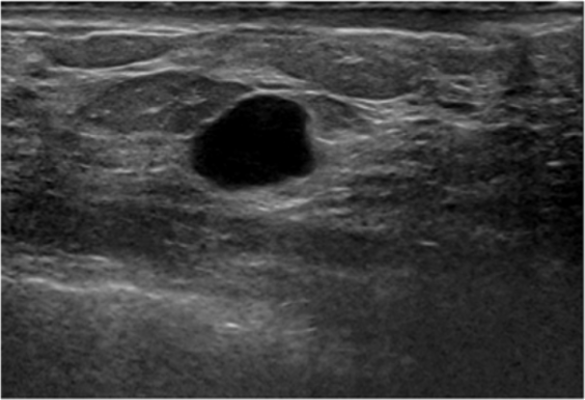
\includegraphics[]{us.png}};
%         \node[below=of us] (gt) {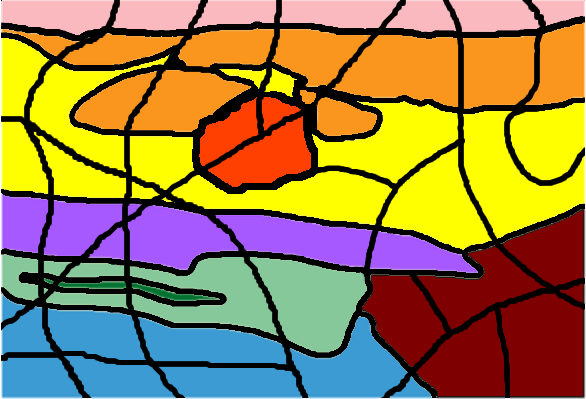
\includegraphics[]{gt.png}};
%       \end{tikzpicture}
%   };

%   \node[right=of problem](data){
%       \begin{tikzpicture}[node distance=3pt, inner sep=0]
%         \node[]           (a){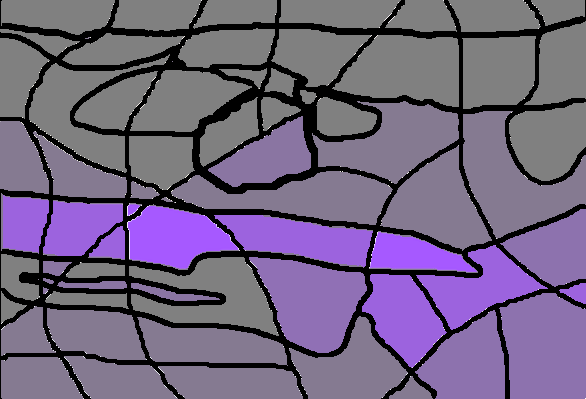
\includegraphics[]{a.png}};
%         \node[below=of a] (b){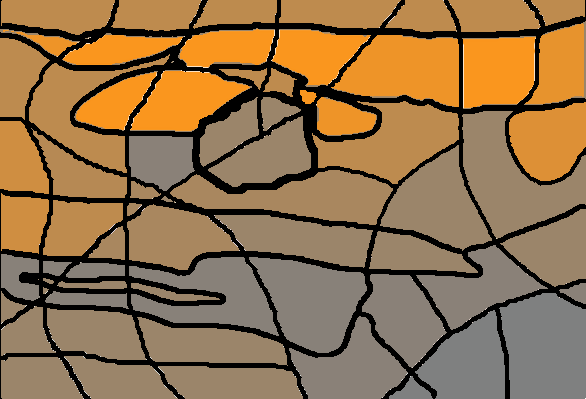
\includegraphics[]{b.png}};
%         \node[right=of a] (c){
\includegraphics[]{c.png}};
%         \node[below=of c] (d){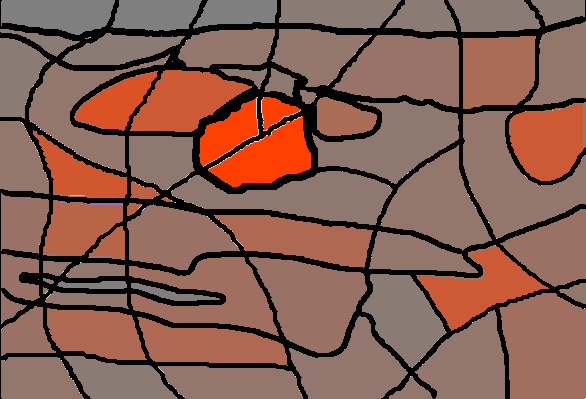
\includegraphics[]{d.png}};
%       \end{tikzpicture}
%   };

%   \node[right=of data](smooth){
%       \begin{tikzpicture}[node distance=3pt, inner sep=0]
%         \node[]           (a){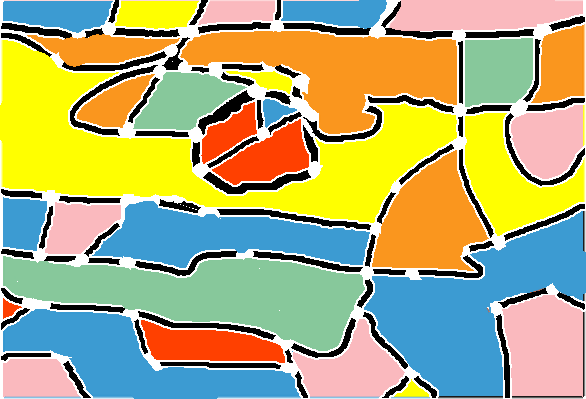
\includegraphics[]{f.png}};
%         \node[below=of a] (b){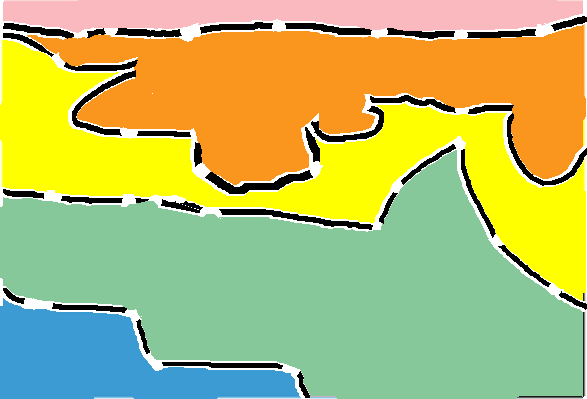
\includegraphics[]{g.png}};
%       \end{tikzpicture}
%   };

%   \node[below=of data](legend){
      \begin{tikzpicture} \begin{customlegend}
        [ legend columns=   5,
          legend style  =   myLegendStyle,
          legend entries= { Background,
            Chest wall,
            Pectoral muscle,
            Adipose tissue,
            Lesion,
            Air (or lungs),
            Rib,
            Fibro-glandular tissue,
            Skin,
            Edge,
          },
        ]

        %  \addMyLegendArea{red}
        \addlegendimage{bgColor!50!black,         fill=bgColor,         area legend}
        \addlegendimage{chestWallColor!50!black,  fill=chestWallColor,  area legend}
        \addlegendimage{pectoralColor!50!black,   fill=pectoralColor,   area legend}
        \addlegendimage{fatColor!50!black,        fill=fatColor,        area legend}
        \addlegendimage{lesionColor!50!black,     fill=lesionColor,     area legend}
        \addlegendimage{lungColor!50!black,       fill=lungColor,       area legend}
        \addlegendimage{ribColor!50!black,        fill=ribColor,        area legend}
        \addlegendimage{fibroGlandColor!50!black, fill=fibroGlandColor, area legend}
        \addlegendimage{skinColor!50!black,       fill=skinColor,       area legend}
        \addlegendimage{boundaryColor!50!black,   fill=boundaryColor,   area legend}
      \end{customlegend} \end{tikzpicture}
  % };

% \end{tikzpicture}
\end{document}


